\documentclass{beamer}
 
\usepackage[american]{babel}
\usepackage[utf8]{inputenc}
\usepackage[T1]{fontenc}
\usepackage{array}
\usepackage{tikz}
\usepackage{epstopdf}
\usetheme{Copenhagen}
\setbeamertemplate{navigation symbols}{}
\title[Audiovisual recognition of drum sequences]{Audiovisual recognition of drum sequences}
\author[A.~Bérard, C.~Robin]{Alexandre Bérard, Charles Robin}

\date{January 10th, 2014}

\newcommand*\oldmacro{}%
\let\oldmacro\insertshorttitle%
\renewcommand*\insertshorttitle{%
  \oldmacro\hfill%
  \insertframenumber\,/\,\inserttotalframenumber}

\begin{document}

    \begin{frame}
    \titlepage
    \end{frame}

    \section{Introduction}    
    \subsection{Database}
    \begin{frame}
        \frametitle{Database}
        \emph{ENST-Drums:} \emph{10 Go} of drum audio and video sequences, played by three different drummers on their own drum kit.
        \vspace*{0.5cm}
       
        Four types of sequence: \emph{hits}, \emph{phrases}, \emph{soli}, \emph{accompaniment}. All sequences are annoted, with the time of each stroke and the corresponding instrument.
        \vspace*{0.5cm}

        Possible instruments: snare drum, bass drum, cymbals (chinese ride, crash, splash, etc.), hi-hat, toms (low tom, mid tom, etc.)
    \end{frame}
    \begin{frame}
        \frametitle{Drum kit}
        \begin{center}
            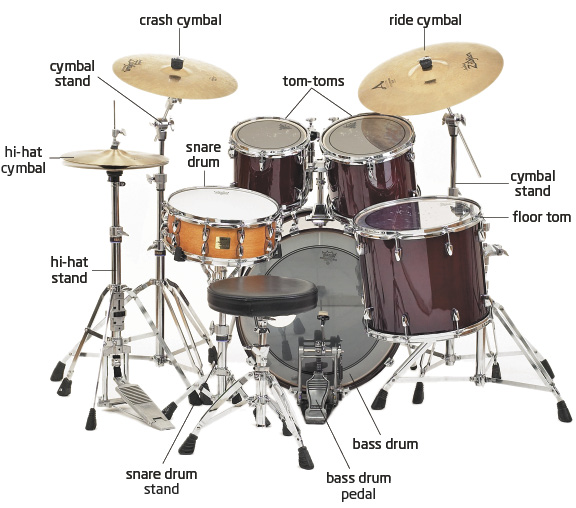
\includegraphics[scale=0.35]{drum-kit.jpg}
        \end{center}
    \end{frame}

    \subsection{Exercise}
    \begin{frame}
        \frametitle{Exercise}
        Different possible classification tasks:
        \begin{itemize}
            \item Recognize the drummer;
            \item Recognize the tool used to hit (stick, brush, mallet);
            \item The instrument that is hit (snare drum, bass drum, etc.);
            \item Or a higher-level category of instrument (e.g. membranes versus plates).
        \end{itemize}
        We could use audio features, video features, or both of them.
    \end{frame}
    \begin{frame}
        \frametitle{Our goal}
        We tried several classification tasks, using audio features. The goal is to recognize the instrument type within four taxonomies.
        \begin{itemize}

            \item \emph{Super-category}: membrane, plate
            \item \emph{Gillet's taxonomy}: bass drum, snare drum, hi-hat (75\% coverage)
            \item \emph{Basic-level}: bass drum, snare drum, tom, cymbal, hi-hat
            \item \emph{Sub-category}: like \emph{basic-level}, but toms are subdivised into low tom, low mid tom, etc., cymbals into splash, ride and crash cymbals.
        \end{itemize}
    \end{frame}
    \subsection{Bibliography}
    \begin{frame}
        \frametitle{Bibliography}
        \footnotesize 
        \nocite{*}
        \bibliographystyle{plain}
        \bibliography{presentation}
        \normalsize
    \end{frame}
    \subsection{Overview}
    \begin{frame}
        \frametitle{Overview}
        \begin{enumerate}
            \item Data segmentation
            \item Feature extraction
            \item Feature selection
            \item Classification
            \item Results and conclusion
        \end{enumerate}
    \end{frame}
    
    \section{Features}
    \subsection{Data segmentation}
    \begin{frame}
        \frametitle{Data segmentation}
        Audio records are sequences of strokes. We must extract those strokes.
        \begin{itemize}
            \item Detect the beginning of each stroke. This process is called \emph{onset detection}. In our case, we use the time defined in the annotations as an oracle.
            \item Define a segment size. It could be either a fixed window (e.g. 200 ms) or the whole audio signal until the next stroke.
            \item We decided that instruments that are played within the same window of 50 ms belong to the same segment.
        \end{itemize}
    \end{frame}
    \subsection{Feature extraction}
    \begin{frame}
        \frametitle{Feature computation}
        \begin{center}
            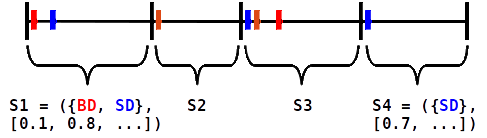
\includegraphics[scale=0.7]{segmentation.png}
        \end{center}
        We used \emph{Yaafe} to compute the features of each audio segment. For each of those features we compute the mean value, with an analysis window of 50 ms, and 50\% overlap.
    \end{frame}
    \begin{frame}
        \frametitle{Feature list}
        \footnotesize 
        \begin{center}
        \begin{tabular}{|c|c|c|}
\hline
Feature&Yaafe name&Dimension\\
\hline
Mel Frequency Cepstrum Coef&MFCC&13\\
\hline
Spectral shape parameters&SpectralShapeStatistics&4\\
\hline
Temporal shape parameters&TemporalShapeStatistics&4\\
\hline
Energy ratio in octave frequency bands&OBSIR&9\\
\hline
Total energy&Energy&1\\
\hline
Zero crossing rate&ZCR&1\\
\hline
Linear prediction coefficients&LPC&6\\
\hline
Spectral flatness&SpectralFlatness&1\\
\hline
Perceptual sharpness&PerceptualSharpness&1\\
\hline
Perceptual spread&PerceptualSpread&1\\
\hline
\end{tabular}
\end{center}
        \normalsize
        We used 3 sets of features : all features (\emph{all}), manually chosen features: mfcc and spectral shape parameters (\emph{manual}), and automatically selected features (\emph{auto}).
        %\begin{itemize}
        %    \item Means of 13 MFCC coefficients (starting by $c_0$).
        %    \item 4 spectral shape parameters: spectral centroïd, width, skewness and kurtosis; defined as \emph{SpectralShapeStatistics} in Yaafe.
        %    \item 
        %\end{itemize}
    \end{frame}
    \subsection{Feature selection}
    \begin{frame}
        \frametitle{Feature selection}
        We used the algorithm \emph{IRMFSP}. Get the attributes that have the maximum inter-classes distance, and minimum intra-class distance. Feature selection is a dimensionality reduction.
        \begin{center}
        \begin{table}
        \caption{First 4 selected attributes}
        \begin{tabular}{|c|c|}
        \hline
        Instrument&Attributes\\
        \hline
        Bass drum&$OBSIR_3$, $OBSIR_2$, $MFCC_0$, $MFCC_1$\\
        \hline
        Snare drum&$OBSIR_2$, $MFCC_2$, $SpecShape_3$, $Spread_0$\\
        \hline
        Hi-hat&$LPC_0$, $TempShape_2$, $MFCC_4$, $OBSIR_8$\\
        \hline
        \end{tabular}
        \end{table}
        \end{center}
    \end{frame}
    \section{Classification}
    \subsection{Classification task}
    \begin{frame}
        \frametitle{Classification task}
        Given a taxonomy with $N$ instruments, determine for each of the instruments, whether it is played in the audio segment or not.
        There are two approaches:
        \begin{itemize}
            \item A single classifier, with $2^N$ classes (one class for each combination of instruments.)
            \item $N$ binary classifiers, which decide if the instrument is played or not.
        \end{itemize}
    \end{frame}
    \subsection{Evaluation protocol}
    \begin{frame}
        \frametitle{Evaluation protocol}
        For both approaches, we tried two classifiers:
        \begin{itemize}
            \item SVM classifier (with RBF kernel) as \emph{Gillet} proposed
            \item K-NN classifier, like \emph{Herrera}, with $k=5$
        \end{itemize}
      
        We used a 10-folds cross-validation.
        We reported, the \emph{precision}, \emph{recall} and \emph{f-score} for each instrument.
        \vspace{0.5cm}
        
        $precision=\frac{correct}{predicted}$,
        $recall=\frac{correct}{true}$,
        $f1=\frac{2\times P\times R}{P+R}$
    \end{frame}
    \subsection{Results}
    \begin{frame}
        \frametitle{Results}
        Results for SVM, with \emph{manual} features:
        \begin{center}
        \footnotesize 
        \begin{table}
        \parbox{.50\linewidth}{       
        \caption{SVM (C=2, $\sigma$=1)}
        \begin{tabular}{|c|c|c|c|}
        \hline
        Instrument&Precision&Recall&F1\\
        \hline
        Bass drum&91.4\%&74.1\%&81.9\%\\
        \hline
        Snare drum&93.0\%&79.6\%&85.8\%\\
        \hline
        Hi-hat&84.7\%&93.2\%&88.8\%\\
        \hline
        Average&89.7\%&82.3\%&85.5\%\\
        \hline
        \end{tabular}
        }
        \hfill
        \parbox{.40\linewidth}{
        \caption{3 SVM (C=2, $\sigma$=1)}
        \begin{tabular}{|c|c|c|}
        \hline
        Precision&Recall&F1\\
        \hline
        90.6\%&76.1\%&82.7\%\\
        \hline
        92.8\%&82.6\%&87.4\%\\
        \hline
        84.7\%&94.1\%&89.2\%\\
        \hline
        89.4\%&84.3\%&86.4\%\\
        \hline
        \end{tabular}
        }
        \end{table}

        \end{center}
    \end{frame}
    
    \begin{frame}
        \frametitle{Results}
        Results for binary SVM and K-NN, with \emph{all} features:
                \begin{center}
        \footnotesize 
        \begin{table}
        \parbox{.50\linewidth}{       
        \caption{3 K-NN (K=5)}
        \begin{tabular}{|c|c|c|c|}
        \hline
        Instrument&Precision&Recall&F1\\
        \hline
        Bass drum&88.5\%&84.9\%&86.6\%\\
        \hline
        Snare drum&91.9\%&90.8\%&91.3\%\\
        \hline
        Hi-hat&91.6\%&92.7\%&92.1\%\\
        \hline
        Average&90.7\%&89.5\%&90.0\%\\
        \hline
        \end{tabular}
        }
        \hfill
        \parbox{.40\linewidth}{
        \caption{3 SVM (C=2, $\sigma$=1)}
        \begin{tabular}{|c|c|c|}
        \hline
        Precision&Recall&F1\\
        \hline
        93.4\%&75.9\%&83.7\%\\
        \hline
        95.5\%&82.3\%&88.4\%\\
        \hline
        84.6\%&97.1\%&90.4\%\\
        \hline
        91.2\%&85.1\%&87.5\%\\
        \hline
        \end{tabular}
        }
        \end{table}  
        \end{center}
    \end{frame}
    
    \begin{frame}
        \frametitle{Results}
        Results for binary SVM, with \emph{all} and \emph{auto} features:
                \begin{center}
                \footnotesize 
        \begin{table}
        \parbox{.50\linewidth}{       
        \caption{3 SVM (\emph{auto})}
        \begin{tabular}{|c|c|c|c|}
        \hline
        Instrument&Precision&Recall&F1\\
        \hline
        Bass drum&86.6\%&86.2\%&86.4\%\\
        \hline
        Snare drum&90.6\%&86.3\%&88.4\%\\
        \hline
        Hi-hat&82.4\%&94.4\%&88.0\%\\
        \hline
        Average&86.5\%&89.0\%&87.6\%\\
        \hline
        \end{tabular}
        }
        \hfill
        \parbox{.40\linewidth}{
        \caption{3 SVM (\emph{all})}
        \begin{tabular}{|c|c|c|}
        \hline
        Precision&Recall&F1\\
        \hline
        93.4\%&75.9\%&83.7\%\\
        \hline
        95.5\%&82.3\%&88.4\%\\
        \hline
        84.6\%&97.1\%&90.4\%\\
        \hline
        91.2\%&85.1\%&87.5\%\\
        \hline
        \end{tabular}
        }
        \end{table}
        \end{center}
    \end{frame}
    \begin{frame}
        \frametitle{Results}
        Average results for SVM, with \emph{manual} features:
        \begin{tabular}{|c|c|c|c|}
        \hline
        Taxonomy&Precision&Recall&F1\\
        \hline
        Gillet(N=3)&89.7\%&82.3\%&85.5\%\\
        \hline
        Basic-level(N=5)&87.7\%&65.8\%&72.7\%\\
        \hline
        Sub-category(N=12)&81.3\%&44.4\%&52.3\%\\
        \hline
        \end{tabular}
    \end{frame}
    \section{Conclusion}
    \begin{frame}
        \frametitle{Remarks}
        In Gillet's thesis, $F1=69.8\%$.
        Our results are comparatively good, because we skipped the \emph{onset detection} step by using an oracle, and our evaluation protocol is less strict.
        \vspace{0.5cm}
        
        There is room for improvement:
        \begin{itemize}
        \item Better feature selection
        \item Parameters tuning
        \item Different type of classifier for each instrument
        \item Use video features.
        \end{itemize}
    \end{frame}
\end{document}
